\documentclass[t]{beamer}
\usepackage[portuges]{babel}
\usepackage[utf8]{inputenc}
\usepackage[T1]{fontenc}
\usepackage{amsmath}
\usepackage{amssymb}
\usepackage{amsfonts}
\usepackage{amsthm}
\usepackage{graphicx}
\usepackage{xcolor}
\usepackage[scaled]{helvet}
\renewcommand{\familydefault}{\sfdefault}
\usepackage{hyperref}
\hypersetup{
	colorlinks=true,
	linkcolor=blue,
	filecolor=magenta,      
	urlcolor=cyan,
	pdftitle={Overleaf Example},
	pdfpagemode=FullScreen,
}
\urlstyle{same}

%%%
%%% Define cores
%%%
\definecolor{cinza}{HTML}{75818B}

%%%
%%% Remove a barra de navegação do Beamer
%%%
\setbeamertemplate{navigation symbols}{}

%%%
%%% Margem dos slides
%%%
\setbeamersize{text margin left=10mm,text margin right=5mm} 

%%%
%%% Redefine a fonte do título dos slides
%%%
\setbeamercolor{frametitle}{fg=cinza}
\setbeamerfont{frametitle}{series=\bfseries}
\setbeamerfont{frametitle}{size=\huge}

%%%
%%% Ajusta a posição do título dos slides e início do texto
%%%
\addtobeamertemplate{frametitle}{\vspace*{2mm}}{\vspace*{5mm}}

%%%
%%% Adiciona páginação nos slides
%%%
%%% Caso não queira, basta comentar este bloco inteiro
%%% para ocultar a paginação
%%%
\addtobeamertemplate{navigation symbols}{}{
\usebeamerfont{footline}
\usebeamercolor[fg]{footline}
}
\setbeamercolor{footline}{fg=cinza}
\setbeamerfont{footline}{series=\bfseries}
\setbeamerfont{footline}{size=\tiny}
\setbeamertemplate{footline}{
\usebeamerfont{page number in head}
\usebeamercolor[fg]{page number in head}
\hspace{5mm}
\insertframenumber/\inserttotalframenumber
\vspace{5mm}
}

%%%
%%% Redefine símbolo padrão do itemize
%%%
\setbeamertemplate{itemize items}[ball]

%%%
%%% Insere numeração nas figuras
%%%
\setbeamertemplate{caption}[numbered]

%%%
%%% Imagem de fundo a ser usada em todos os slides (exceto
%%% no primeiro e no último)
%%%
\usebackgroundtemplate
{

\includegraphics[width=\paperwidth,height=\paperheight]{fundo.png}
}

%%%
%%% Adiciona slide de "Estrutura"
%%%
%\AtBeginSection[]{\frame{\frametitle{Estrutura}\tableofcontents
%[current]}}

%%%
%%% Define fontes e cores do slide de "Estrutura"
%%%
\setbeamerfont{section in toc}{series=\bfseries}
\setbeamercolor{section in toc}{fg=gray}
\setbeamerfont{section in toc shaded}{series=\mdseries}
\setbeamercolor{section in toc shaded}{fg=gray!01}
\setbeamercolor{subsection in toc}{fg=cinza}
\setbeamercolor{subsection in toc shaded}{fg=gray!60}
\setbeamercolor{subsubsection in toc}{fg=cinza}
\setbeamercolor{subsubsection in toc shaded}{fg=gray!60}

\usepackage{listings}
\definecolor{codegreen}{rgb}{0,0.6,0}
\definecolor{codegray}{rgb}{0.5,0.5,0.5}
\definecolor{codepurple}{rgb}{0.58,0,0.82}
\definecolor{backcolour}{rgb}{0.95,0.95,0.92}

\lstdefinestyle{mystyle}{
	backgroundcolor=\color{backcolour},   
	commentstyle=\color{codegreen},
	keywordstyle=\color{magenta},
	numberstyle=\tiny\color{codegray},
	stringstyle=\color{codepurple},
	basicstyle=\ttfamily\footnotesize,
	breakatwhitespace=false,         
	breaklines=true,                 
	captionpos=b,                    
	keepspaces=true,                 
	numbers=left,                    
	numbersep=5pt,                  
	showspaces=false,                
	showstringspaces=false,
	showtabs=false,                  
	tabsize=2
}

\lstset{style=mystyle}

\mode<presentation>
%%%
%%% Início
%%%
\begin{document}

%%%
%%% Slide da capa
%%%
{
	\usebackgroundtemplate{
\includegraphics[width=\paperwidth]{capa.png}}
	\begin{frame}[plain]
		\vspace{18mm}
		%%%
		%%% Título da Apresentação
		%%%
		\begin{flushright}
			\textcolor{cinza}{\textbf{\huge{
				Flask
			}}}
		\end{flushright}
		
		\vspace{-6mm}
		%%%
		%%% Nome do autor
		%%%
		\begin{flushright}
			\textcolor{cinza}{\textbf{\scriptsize{
				Sadi Jr.
			}}}
		\end{flushright}
		
		\vspace{-7mm}
		%%%
		%%% Formação | Departamento | Centro
		%%%
		\begin{flushright}
			\textcolor{cinza}{\scriptsize{
				Sistemas de Informação | Departamento de Informática e Estatística | Centro Tecnológico
			}}
		\end{flushright}
		
		
	\end{frame}
}

%%%
%%% Demais slides (exceto o slide final)
%%%
\begin{frame}
	\frametitle{Conteúdo}
	\tableofcontents
\end{frame}

\section{O que é Flask?}
\section{O que é um \textit{Microframework}?}
\section{De volta ao Flask}
\section{Por que usar?}
\section{Werkzeug}
\section{Jinja 2}
\section{Flask \textit{vs} Django}
\section{Referências}

\begin{frame}
	\frametitle{O que é Flask?}
	\begin{figure}[!ht]
		\centering
		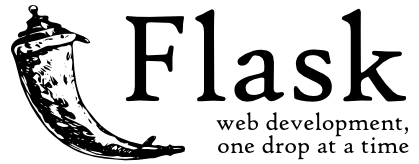
\includegraphics[scale=.4]{flask.png}
	\end{figure}
	
	Flask é um \textit{microframework} Python para desenvolvimento \textit{web}, baseado no  \href{https://werkzeug.palletsprojects.com/en/2.0.x/}{Werkzeug}, \href{https://jinja.palletsprojects.com/en/3.0.x/}{Jinja 2} e em Boas Intenções (``Good Intentions'').
	\vspace{1cm}
  
	Flask pode ser ``micro'', mas está pronto para ser usado em produção, preenchendo uma gama variada de necessidades.
\end{frame}

\begin{frame}
	\frametitle{O que é \textit{Microframework}?}
	Um \textit{microframework} é um \textit{framework} modularizado que possui uma estrutura inicial muito mais simples quando comparado a um \textit{framework} convencional. 
	\vspace{.5cm}
	
	Em outras palavras, um \textit{microframework} é uma versão minimalista de um \textit{framework}.
\end{frame}

\begin{frame}
	\frametitle{De volta ao Flask}
	Flask, por ser um \textit{microframework}, procura manter o núcleo simples, mas extensível, não possuindo soluções pré-prontas, permitindo ao desenvolvedor decidir quais ferramentas deseja usar ao mesmo tempo em que permite dispensar ferramentas não necessárias.
	\vspace{.5cm}
	
	Por padrão, o Flask não inclui uma camada de abstração de banco de dados, validação de formulário, ou qualquer outra coisa para a qual já existam diferentes bibliotecas. Em vez disso, suporta extensões para adicionar uma determinada funcionalidade à sua aplicação como se ela tivesse sido implementada no Flask em si. Muitas extensões fornecem integração de banco de dados, validação de formulários, manipulação de \textit{upload}, diversas tecnologias de autenticação abertas, entre outros.
\end{frame}

\begin{frame}
	\frametitle{Por que usar?}
	Flask é a solução ideal para que busca:
	\vspace{.5cm}
	
	\begin{itemize}
		\item Simplicidade: Por possuir apenas o necessário para o desenvolvimento de uma aplicação, um projeto escrito com Flask é mais simples se comparado aos \textit{frameworks} maiores, já que a quantidade de arquivos é muito menor e sua arquitetura é muito mais simples. 
		\vspace{.5cm}
		
		\item Rapidez no desenvolvimento: Com o Flask, o desenvolvedor se preocupa em apenas desenvolver o necessário para um projeto, sem a necessidade de realizar configurações que muitas vezes não são utilizadas.
	\end{itemize}
\end{frame}

\begin{frame}
	\frametitle{Por que usar?}
	\begin{itemize}
		\item Soluções para projetos pequenos: Por possuir uma arquitetura muito simples (um único arquivo inicial) os projetos escritos em Flask tendem a ser menores e mais leves se comparados a \textit{frameworks} maiores. 
		
		\vspace{.5cm}
		\item Aplicações robustas: Apesar de ser um \textit{microframework}, o Flask permite a criação de aplicações robustas, já que é totalmente personalizável, permitindo, caso necessário, a criação de uma arquitetura mais definida. 
	\end{itemize}		  
\end{frame}

\begin{frame}
	\frametitle{Werkzeug}
	 Biblioteca para desenvolvimento de aplicações WSGI \textit{(Web Server Gateway Interface)}, que é a especificação universal de como deve ser a interface entre uma aplicação Python e \textit{um web server}. 
	 \vspace{.5cm}
	 
	 Ela possui a implementação básica deste padrão para interceptar \textit{requests} e lidar com \textit{responses}, controle de cache, \textit{cookies}, \textit{status HTTP}, roteamento de \textit{URLs} e também conta com uma poderosa ferramenta de \textit{debug}.
\end{frame}

\begin{frame}
	\frametitle{Jinja 2}
	Linguagem de modelos (\textit{template language}) responsável pela renderização de páginas HTML dinâmicas, ao utilizar marcações.
	
	\lstinputlisting{template.html}
\end{frame}

\begin{frame}
	\frametitle{Flask \textit{vs} Django}
	\begin{table}[]
		\begin{tabular}{|c|c|}
			\hline
			Flask & Django\\\hline
			Desenvolvimento rápido e & Desenvolvimento rápido e\\
			fácil de aplicações & escalável de aplicações maiores\\\hline
			Curva curta de aprendizado & Curva mais longa de aprendizado\\\hline
			Minimalista, simples e & Estrutura completa\\
			muito flexível & e padronizada\\\hline
			Facilidade de adicionar  & Diversos componentes\\
			extensões & já prontos\\\hline
			Aplicações mais flexíveis, & Aplicações mais complexas,\\
			simples e leves & robustas e escaláveis\\\hline
			Menor comunidade & Maior comunidade\\\hline
		\end{tabular}
	\end{table}
\end{frame}

\begin{frame}
	\frametitle{Referências}
	\begin{itemize}
		\item \url{https://flask.palletsprojects.com/en/2.0.x/}
		\item \url{https://www.treinaweb.com.br/blog/o-que-e-flask}
		\item \url{https://werkzeug.palletsprojects.com/en/2.0.x/}
		\item \url{https://jinja.palletsprojects.com/en/3.0.x/}
		\item \url{https://en.wikipedia.org/wiki/Web\_Server\_Gateway\_Interface}
	\end{itemize}
\end{frame}
%%%
%%% Slide final
%%%
{
	\usebackgroundtemplate{
\includegraphics[width=\paperwidth]{capa.png}}
	\begin{frame}[plain]
		\vspace{15mm}
		\begin{center}
			\textcolor{cinza}{
				\textbf{Contato}
			}
		\end{center}
		\vspace{-6mm}
		\begin{center}
			\textcolor{cinza}{\scriptsize{
				E-mail: sadijacinto@gmail.com
			}}
		\end{center}
		\vspace{-6mm}
		\begin{center}
			\textcolor{cinza}{\scriptsize{
				Github: github.com/SadiJr
			}}
		\end{center}
	\end{frame}
}
\end{document}
